\section{Floquet theory}

Since we describe the lifetime of an electron in certain Landau level using conventianal perturbation theeory, now we can apply the Floquet theory to identify the difference of these methods.

\noindent
First we need to identify the \textit{quasienergies} and periodic \textit{Floquet modes} for derived wavefunctions \eqref{1.52} for a 2DEG system with both stationary magnetic field and strong dressing filed.

\noindent
Let's consider the following paramter which is lineraly increasing in time
\begin{equation} \label{3.1}
  \Delta_E t \equiv \frac{t}{T} \int_0^T dt' \; L(\zeta,\dot{\zeta},t')
\end{equation}
where we can calculate this using Eq. \eqref{1.42} and \eqref{1.51} as follows
\begin{equation} \label{3.2}
  \begin{aligned}
    \Delta_E t =
    \frac{t}{T} \int_0^T dt' \;
    \frac{1}{2}m_e \frac{(eE\omega)^2}{m_e^2(\omega_0^2 - \omega^2)^2} \cos[2](\omega t')
    & - \frac{1}{2}m_e\omega_0^2 \frac{(eE)^2}{m_e^2(\omega_0^2 - \omega^2)^2} \sin[2](\omega t') \\
    & +
    \frac{eE}{m_e(\omega_0^2 - \omega^2)} \sin(\omega t') eE \sin(\omega t')
  \end{aligned}
\end{equation}
\begin{equation} \label{3.3}
  \begin{aligned}
    \Delta_E t  =
    \frac{t\omega}{2\pi} \times
    \frac{(eE)^2}{2m_e(\omega_0^2 - \omega^2)^2}
    \bigg[
    \omega^2
    \int_0^T dt' \; \cos[2](\omega t')
    & -
    \omega_0^2
    \int_0^T dt'\; \sin[2](\omega t') \\
    & +
    2(\omega_0^2 - \omega^2) \int_0^T dt'\; \sin[2](\omega t')
    \bigg]
  \end{aligned}
\end{equation}
\begin{equation} \label{3.4}
  \begin{aligned}
    \Delta_E t  =
    \frac{t\omega}{2\pi} \times
    \frac{(eE)^2}{2m_e(\omega_0^2 - \omega^2)^2}
    \bigg[
    \omega^2
    \frac{\pi}{\omega}
    -
    \omega_0^2
    \frac{\pi}{\omega}
    +
    2(\omega_0^2 - \omega^2) \frac{\pi}{\omega}
    \bigg]
  \end{aligned}
\end{equation}
\begin{equation} \label{3.5}
  \begin{aligned}
    \Delta_E t  =
    \frac{t\omega}{2} \times
    \frac{(eE)^2}{2m_e(\omega_0^2 - \omega^2)^2}
    (\omega_0^2 - \omega^2) =
    \frac{(eE)^2}{4m_e(\omega_0^2 - \omega^2)} t
  \end{aligned}
\end{equation}
Since this is the continuous increasing part of the Laggrangian integral in Eq. \eqref{1.52} we can make this as $2\omega$ periodic function as follows
\begin{equation} \label{3.6}
    \Lambda\equiv
    \int_0^t dt' \; L(\zeta,\dot{\zeta},t') -
    \frac{t}{T} \int_0^T dt' \; L(\zeta,\dot{\zeta},t')
\end{equation}
which can be proved as follows. First consider the first term of the $\Lambda$
\begin{equation} \label{3.7}
  \begin{aligned}
    \int_0^t dt' \; L(\zeta,\dot{\zeta},t') =
    \frac{(eE)^2}{2m_e(\omega_0^2 - \omega^2)^2}
    \bigg[
    \omega^2
    \int_0^t dt' \; \cos[2](\omega t')
    & -
    \omega_0^2
    \int_0^t dt'\; \sin[2](\omega t') \\
    & +
    2(\omega_0^2 - \omega^2) \int_0^t dt'\; \sin[2](\omega t')
    \bigg]
  \end{aligned}
\end{equation}
\begin{equation} \label{3.8}
  \begin{aligned}
    \int_0^t dt' \; L(\zeta,\dot{\zeta},t') =
    \frac{(eE)^2}{2m_e(\omega_0^2 - \omega^2)^2}
    \bigg[
    \omega^2
    \qty[\frac{t}{2} + \frac{\sin(2\omega t)}{4\omega}]
    & -
    \omega_0^2
    \qty[\frac{t}{2} - \frac{\sin(2\omega t)}{4\omega}] \\
    & +
    2(\omega_0^2 - \omega^2)
    \qty[\frac{t}{2} - \frac{\sin(2\omega t)}{4\omega}]
    \bigg]
  \end{aligned}
\end{equation}
\begin{equation} \label{3.9}
  \begin{aligned}
    \int_0^t dt' \; L(\zeta,\dot{\zeta},t')  =
    \frac{(eE)^2}{2m_e(\omega_0^2 - \omega^2)^2}
    \bigg[&
    \frac{t}{2}
    \qty[\omega^2 - \omega_0^2 + 2\omega_0^2 - 2\omega^2] \\
    & +
    \frac{\sin(2\omega t)}{4\omega}
    \qty[\omega^2 + \omega_0^2 - 2\omega_0^2 + 2\omega^2]
    \bigg]
  \end{aligned}
\end{equation}
\begin{equation} \label{3.10}
    \int_0^t dt' \; L(\zeta,\dot{\zeta},t')  =
    \frac{(eE)^2}{4m_e(\omega_0^2 - \omega^2)}t
    +
    \frac{(eE)^2\qty(3\omega^2 - \omega_0^2)}{8m_e\omega(\omega_0^2 - \omega^2)^2}
    \sin(2\omega t)
\end{equation}
then using Eq.\eqref{3.5} we can write this as
\begin{equation} \label{3.11}
    \int_0^t dt' \; L(\zeta,\dot{\zeta},t')  =
    \Delta_E t
    +
    \frac{(eE)^2\qty(3\omega^2 - \omega_0^2)}{8m_e\omega(\omega_0^2 - \omega^2)^2}
    \sin(2\omega t).
\end{equation}
Now we can express
\begin{equation} \label{3.12}
    \Lambda  =
    \Delta_E t
    +
    \frac{(eE)^2\qty(3\omega^2 - \omega_0^2)}{8m_e\omega(\omega_0^2 - \omega^2)^2}
    \sin(2\omega t) - \Delta_E t
    =
    \frac{(eE)^2\qty(3\omega^2 - \omega_0^2)}{8m_e\omega(\omega_0^2 - \omega^2)^2} \sin(2\omega t)
\end{equation}
which is a periodic function in time with $2\omega$ frequency.

\noindent
Now using this parmaters we can factorize the wavefunction \eqref{1.52} as linearly time dependend part and periodic time dependend part as follows
\begin{equation} \label{3.13}
  \begin{aligned}
    \psi_{\alpha}(x,y,t)  = &
    \exp(\frac{i}{\hbar}\qty[-E_nt + \Delta_E t ])
    \frac{1}{\sqrt{L_x}} \chi_n\big(y - \zeta(t)\big)
    \\
    & \times
    \exp(
     \frac{i}{\hbar}\bigg[
     p_x x +
     \frac{eEy}{\omega}\cos(\omega t)+
     m_e\dot{\zeta(t)}\big[y-\zeta(t)\big]
     + \int_0^{t}dt'L(\zeta,\dot{\zeta},t') - \Delta_E t  \bigg])
  \end{aligned}
\end{equation}
where we can identify(let $\alpha \rightarrow (n,m)$) the \textit{quasienergies} as
\begin{equation} \label{3.14}
  \varepsilon_{\alpha} \equiv
  \varepsilon_{n} =
  \hbar \omega_0\qty(n + \frac{1}{2}) - \Delta_E \quad \text{where} \quad
  n = 0,1,2, ... \quad \text{for any given } m
\end{equation}
which is only depend on one quantum number ($n$) and \textit{Floquet modes} as
\begin{equation} \label{3.15}
  \begin{aligned}
    \phi_{\alpha}(x,\tilde{y},t) \equiv &
    \frac{1}{\sqrt{L_x}} \chi_{n}\big(\tilde{y} - \zeta(t)\big)
    \exp(
     \frac{i}{\hbar}\bigg[
     p_x x +
     \frac{eE\tilde{y}}{\omega}\cos(\omega t)+
     m_e\dot{\zeta}(t)\big[\tilde{y}-\zeta(t)\big]
     + \Lambda \bigg])
  \end{aligned}
\end{equation}
with
\begin{equation} \label{3.16}
  \zeta(t) = \frac{eE}{m_e(\omega_0^2 - \omega^2)}\sin(\omega t) \quad \text{and} \quad
  \dot{\zeta}(t) = \frac{eE\omega}{m_e(\omega_0^2 - \omega^2)}\cos(\omega t)
\end{equation}
where  \textit{Floquet modes} are time-periodic functions that also create a complete orthonormal set.
\hfill$\blacksquare$
\begin{figure}[ht!]
  \centering
  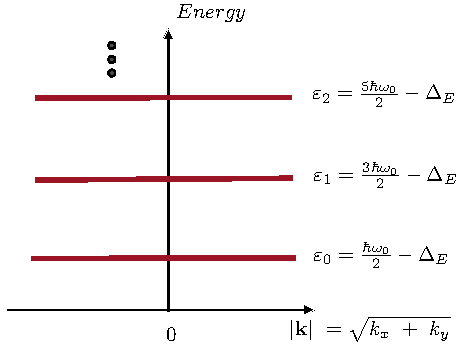
\includegraphics[scale=0.9]{figures/fig03.pdf}
  \caption{Quasienergies for each Landau levels against magnitude of momentum.}
  \label{fig:3.0}
\end{figure}

\vspace{5mm}
\noindent
Therefore using Floquet theory, the solutions (Floquet states) for the periodic Hamiltonian \eqref{1.5} can be written in position space as
\begin{equation} \label{3.17}
  \psi_{\alpha}(x,\tilde{y},t) =
  \exp(-\frac{i}{\hbar}\varepsilon_{\alpha}t)   \phi_{\alpha} (x,\tilde{y},t)
\end{equation}
where
\begin{equation} \label{3.18}
  \varepsilon_{\alpha} \equiv
  \qty(\frac{eB\hbar }{m_e})\qty(n + \frac{1}{2}) -
  \frac{(eE)^2}{4m_e(\omega_0^2 - \omega^2)}
  \quad \text{where} \quad
  n = 0,1,2, ...
\end{equation}
and
\begin{equation} \label{3.19}
  \begin{aligned}
    \phi_{\alpha}(x,\tilde{y},t) \equiv &
    \frac{1}{\sqrt{L_x}}
    \chi_{n}\qty(\tilde{y} - \frac{eE\sin(\omega t)}{m_e(\omega_0^2 - \omega^2)} ) \\
    & \times
    \exp(
     \frac{i}{\hbar}\qty[
     p_x x +
     \frac{eE\tilde{y}}{\omega}\cos(\omega t)+
     \frac{eE\omega \tilde{y} }{(\omega_0^2 - \omega^2)}\cos(\omega t)
     ])\\
     & \times
     \exp(\frac{i}{\hbar}\qty[
     -\frac{(eE)^2\omega }{2m_e(\omega^2 - \omega_0^2)^2}\sin(2\omega t)
     + \frac{(eE)^2\qty(3\omega_0^2 - \omega^2)}{8m_e\omega(\omega_0^2 - \omega^2)^2} \sin(2\omega t)
  ])
  \end{aligned}
\end{equation}

\noindent
Now we can write this by more simplying and considering spacial dependencies and using previous subtituting done in Eq. \eqref{1.16} and now $\chi$ function depend on both quantum numbers because $y_0$ gives the $p_x$ dependence and we can present as
\begin{equation} \label{3.20}
  \begin{aligned}
    \phi_{\alpha}(x,y,t)  \equiv
    \frac{1}{\sqrt{L_x}}
    \chi_{n}\qty(y - y_0 - \frac{eE\sin(\omega t)}{m_e(\omega_0^2 - \omega^2)} ) &
    \exp( \frac{i p_x }{\hbar}x )
    \exp(
     \frac{i}{\hbar}
     \qty[
     \frac{eE\omega_0^2\cos(\omega t)}{\omega(\omega_0^2 - \omega^2)}]
     \qty(y - y_0 ))\\
     & \times
     \exp(\frac{-i}{\hbar}
     \qty[
     \frac{(eE)^2\qty(\omega_0^2 + \omega^2)}{8\omega m_e(\omega_0^2 - \omega^2)^2}
     ]\sin(2\omega t)
     )
  \end{aligned}
\end{equation}

\noindent
Now we can transform this solution in spacial variable into the momentum space using Fourier trasform over the considering confined space $A=L_xL_y$.
\begin{equation} \label{3.21}
  \begin{aligned}
    \phi_{\alpha}(k_x,k_y,t)  &=
    \int_{-L_y/2}^{L_y/2} dy\; \exp(-ik_y y)
    \qty[
    \frac{1}{\sqrt{L_x}}
    \chi_{n}\qty(y - y_0 - \frac{eE\sin(\omega t)}{m_e(\omega_0^2 - \omega^2)} )
    \exp(
     \frac{i}{\hbar}
     \qty[
     \frac{eE\omega_0^2\cos(\omega t)}{\omega(\omega_0^2 - \omega^2)}]
     y)] \\
     & \times
     \int_{-L_x/2}^{L_x/2} dx\; \exp(-ik_x x)
     \qty[
     \exp( \frac{i p_x }{\hbar}x )
     ] \\
     &
     \times
     \exp(
      \frac{-i}{\hbar}
      \qty[
      \frac{eE\omega_0^2\cos(\omega t)}{\omega(\omega_0^2 - \omega^2)}]y_0)
      \times
     \exp(\frac{-i}{\hbar}
     \qty[
     \frac{(eE)^2\qty(\omega_0^2 + \omega^2)}{8\omega m_e(\omega_0^2 - \omega^2)^2}
     ]\sin(2\omega t)
     )
  \end{aligned}
\end{equation}
Then this can be re-write as follows
\begin{equation} \label{3.22}
    \phi_{\alpha}(k_x,k_y,t)  =
    \exp(
     \frac{-i}{\hbar}
     \qty[
     \frac{eE\omega_0^2\cos(\omega t)}{\omega(\omega_0^2 - \omega^2)}]y_0)
    \exp(\frac{-i}{\hbar}
    \qty[
    \frac{(eE)^2\qty(\omega_0^2 + \omega^2)}{8\omega m_e(\omega_0^2 - \omega^2)^2}
    ]\sin(2\omega t))
    \Theta_{\alpha}(k_y,t)
    \delta_{k_x,\frac{p_x}{\hbar}}
\end{equation}
where we used
\begin{equation} \label{3.23}
  \int_{L_x} dx\;
  \exp( -ik_x x + \frac{i p_x }{\hbar}x ) =
  L_x \delta_{k_x,\frac{p_x}{\hbar}}
\end{equation}
and
\begin{equation} \label{3.24}
  \Theta_{\alpha}(k_y,t) \equiv
  \int_{-L_y/2}^{L_y/2}  dy\; \exp(-ik_y y)
  \qty[
  \sqrt{L_x}
  \chi_{n}\qty(y -y_0 - \frac{eE\sin(\omega t)}{m_e(\omega_0^2 - \omega^2)} )
  \exp(
   \frac{i}{\hbar}
   \qty[
   \frac{eE\omega_0^2\cos(\omega t)}{\omega(\omega_0^2 - \omega^2)}]
   y)]
\end{equation}
and this can be simplied as
\begin{equation} \label{3.25}
  \Theta_{\alpha}(k_y,t) =
  \sqrt{L_x}
  \int_{-L_y/2}^{L_y/2} dy\;
  \chi_{n}\qty(y -y_0 - \frac{eE\sin(\omega t)}{m_e(\omega_0^2 - \omega^2)} )
  \exp(
    -ik_y y +
   \frac{i}{\hbar}
   \qty[
   \frac{eE\omega_0^2\cos(\omega t)}{\omega(\omega_0^2 - \omega^2)}] y).
\end{equation}
Then by defining
\begin{equation} \label{3.26}
  \mu(t) \equiv \frac{eE\sin(\omega t)}{m_e(\omega_0^2 - \omega^2)} + y_0
\end{equation}
and
\begin{equation} \label{3.27}
  \gamma(t) \equiv
  \frac{eE\omega_0^2\cos(\omega t)}{\hbar\omega(\omega_0^2 - \omega^2)}
\end{equation}
we can re-write this by neglecting time dependencies as
\begin{equation} \label{3.28}
  \Theta_{\alpha}(k_y,t) =
  \sqrt{L_x}
  \int_{-\infty}^{\infty} dy\;
  \chi_{n}\qty(y - \mu )
  \exp(
    -i\qty(k_y - \gamma)
    y).
\end{equation}
We can subtitute following variables
\begin{equation} \label{3.29}
  {k_y}' = k_y -\gamma \quad \text{and} \quad y' = y -\mu
\end{equation}
and for $L_y \rightarrow \infty$ this leads to
\begin{equation} \label{3.30}
  \Theta_{\alpha}({k_y}' ,t) =
  {\sqrt{L_x}} e^{-i {k_y}'\mu}
  \int_{-\infty}^{\infty} dy'\;
  \chi_{n}\qty(y')
  \exp(-i{k_y}' y')
  =
  {\sqrt{L_x}} e^{-i {k_y}'\mu}
  \sqrt{\kappa}
  \int_{-\infty}^{\infty} dy'\;
  \vartheta_n \qty(\kappa y')
  \exp(-i{k_y}' y')
\end{equation}
We know that $\{\chi_{\alpha}\}$ are well-known harmonic eigenfunctions(with Gauss-Hermite functions) as given in the Eq. \eqref{1.47}. However, the equation in \eqref{3.30} represents the Fourier transform of the these Gauss-Hermite functions. Due to the symmetric condition [*Ref:E.Celeghini] the Fourier transform of these functions can be represent as
\begin{equation} \label{3.31}
  \mathcal{FT}[\vartheta_n(\kappa x),x,k] = \frac{i^n}{|\kappa|}\vartheta_n(k/\kappa)
\end{equation}
Therefore
\begin{equation} \label{3.32}
  \Theta_{\alpha}({k_y}' ,t) =
  \sqrt{L_x}e^{-i {k_y}'\mu} \times \frac{i^n}{\sqrt{\kappa}} \vartheta_n \qty(\frac{{k_y}'}{\kappa}) =
    \sqrt{L_x}e^{-i {k_y}'\mu}
    \tilde{\chi}_{n}\qty({k_y}')
\end{equation}
where
\begin{equation} \label{3.33}
  \tilde{\chi}_{n}\qty(k) =
  \frac{i^n}{\sqrt{2^{n} n! \sqrt{\pi}}}
  \qty(\frac{1}{\kappa})^{1/2}
  e^{-\frac{k^2}{2 \kappa^2}}
  \mathcal{H}_{\alpha} \qty(\frac{k}{\kappa}).
\end{equation}
Using Eq. \eqref{3.32} and Eq. \eqref{3.22} we can derive that
\begin{equation} \label{3.34}
  \begin{aligned}
    \phi_{\alpha}(k_y,t)  =
    \exp(
      \frac{-i}{\hbar}
      \qty[
      \frac{eE\omega_0^2\cos(\omega t)}{\omega(\omega_0^2 - \omega^2)}]y_0
    )&
    \exp(
      \frac{-i}{\hbar}
      \qty[
      \frac{(eE)^2\qty(\omega_0^2 + \omega^2)}{8\omega m_e(\omega_0^2 - \omega^2)^2}
      ]\sin(2\omega t)
    )
    \\
    & \times
    {\sqrt{L_x}} e^{-i \qty(k_y -\gamma)\mu}
    \tilde{\chi}_{n}\qty(k_y -\gamma)
  \end{aligned}
\end{equation}
where we included the $k_x$ dependence into $\alpha$ quantum number using $m$ value and this can be re-write subtituting $\mu$ and $\gamma$ values as follows
\begin{equation} \label{3.35}
  \begin{aligned}
    \phi_{\alpha}(k_y,t) & =
    {\sqrt{L_x}}
    \exp(
      \frac{-i}{\hbar}
      \qty[
      \frac{eE\omega_0^2\cos(\omega t)}{\omega(\omega_0^2 - \omega^2)}]y_0
    )
    \exp(
      \frac{-i}{\hbar}
      \qty[
      \frac{(eE)^2\qty(\omega_0^2 + \omega^2)}{8\omega m_e(\omega_0^2 - \omega^2)^2}
      ]\sin(2\omega t)
    ) \\
    & \times
    \exp(
      -ik_y  \frac{eE\sin(\omega t)}{m_e(\omega_0^2 - \omega^2)}
    )
    \exp(
      \frac{i}{\hbar}
      \qty[ \frac{eE\omega_0^2\cos(\omega t)}{\omega(\omega_0^2 - \omega^2)}]
      \frac{eE\sin(\omega t)}{m_e(\omega_0^2 - \omega^2)}
    )
    \exp(
      -i k_y y_0
    ) \\
    & \times
    \exp(
      i \frac{1}{\hbar}
      \qty[ \frac{eE\omega_0^2\cos(\omega t)}{\omega(\omega_0^2 - \omega^2)}]
      y_0
    )
    \tilde{\chi}_{n}\qty(k_y -\gamma)
  \end{aligned}
\end{equation}
and
\begin{equation} \label{3.36}
  \begin{aligned}
    \phi_{\alpha}(k_y,t) & =
    {\sqrt{L_x}}
    \exp(
      \frac{i}{\hbar}
      \qty[
      \frac{(eE)^2\qty(3\omega_0^2 - \omega^2)}{8\omega m_e(\omega_0^2 - \omega^2)^2}
      ]\sin(2\omega t)
    ) \\
    & \times
    \exp(
      -ik_y  \qty[\frac{eE\sin(\omega t)}{m_e(\omega_0^2 - \omega^2)} + y_0]
    )
    \tilde{\chi}_{n}\qty(k_y -\gamma).
  \end{aligned}
\end{equation}
For notation convinient we can introduce few constant as follows
\begin{equation} \label{3.37}
  b \equiv
  \frac{(eE)^2\qty(3\omega_0^2 - \omega^2)}{8\hbar \omega m_e(\omega_0^2 - \omega^2)^2}
\end{equation}
and
\begin{equation} \label{3.38}
  d \equiv
  \frac{eE}{m_e(\omega_0^2 - \omega^2)}
\end{equation}
with
\begin{equation} \label{3.39}
  g \equiv
  \frac{eE\omega_0^2}{\hbar\omega(\omega_0^2 - \omega^2)}.
\end{equation}
Therefore we can write Eq. \eqref{3.36} as
\begin{equation} \label{3.40}
  \begin{aligned}
    \phi_{\alpha}(k_y,t) & =
    {\sqrt{L_x}}
    e^{
      ib\sin(2\omega t)
    }
    e^{
      -ik_y  \qty[d\sin(\omega t) + y_0]
    }
    \tilde{\chi}_{n}\qty(k_y -g\cos(\omega t)).
  \end{aligned}
\end{equation}
